%%%%%%%%%%%%%%%%%%%%%%%%%%%%%%%%%%%%%%%%%%%%%%%%%%%%%%%%%%%

\chapter{Modello del sistema - gruppo 3}
\label{ref:modSistemaGruppo3}

%%% Il gruppo 3 scriverà il suo modello del sistema. Esso dovrà includere: attori, casi d'uso (descrizione e tabella), scenari, diagrammi dei casi d'uso, diagrammi di sequenza, diagramma delle attività, screen mockups della funzionalità %%%

\section{Attori}
<Gli attori della funzionalità Media sono in comune agli altri gruppi>.

\section{Scenari}
\begin{comment}
Inserire qui gli scenari che sono un'istanza dei casi d'uso: gli scenari danno dei valori al flusso degli eventi dei casi d'uso. Esempio di caso d'uso "visualizza libretto": l'utente Antonio - che ha effettuato il login con username "Antonio" e password "antonioilmigliore" - accede alla sezione "libretto" e visualizza gli esami sostenuti Programmazione e Inglese con le votazioni rispettive di 25 e 30.
\end{comment}
\subsection{Simulazione della media}

Lo studente Giuseppe Crincoli, dopo aver effettuato il login, seleziona la funzionalità Previsione Media, seleziona simulazione con esami, successivamente, il sistema mostra gli esami di Ingegneria Del Software, Calcolo Numerico e Algoritmi, il quale seleziona gli esami di Ingegneria Del Software e Calcolo Numerico, inserisce la votazione di 26/30 per l'esame di Ingegneria Del Software e 23/30 per l'esame di Calcolo Numerico, il sistema restituisce la previsione media aritmetica con valore di 24,5, la previsione media ponderata con valore di 24,8 e base di laurea con votazione di 91/110.

\subsection{Simulazione della media con valori non validi o vuoti}

Lo studente Emilio Fabrizio, dopo aver effettuato il login, seleziona la funzionalità Previsione Media, seleziona simulazione con esami, successivamente, il sistema mostra gli esami di Ingegneria Del Software, Calcolo Numerico e Algoritmi, lo studente inserisce il voto di 15/30 riguardante l'esame di Calcolo Numerico oppure non inserisce un voto per nessun esame e preme sul tasto calcola media, il sistema mostra il seguente messaggio: "Non è possibile effettuare nessuna previsione".

\subsection{Esami da conseguire terminati}

Lo studente Gianluca Di Cristino, dopo aver effettuato il login, seleziona la funzionalità Previsione Media, seleziona simulazione con esami, il sistema mostra la carriera completa allo studente, lo studente non può selezionare alcun esame poichè ha conseguito tutti gli esami, il sistema mostra il seguente messaggio: "Non è possibile effettuare nessuna previsione". 

\subsection{Mancata connessione}

La studentessa Giovanna D'Ercole, dopo aver effettuato il login, seleziona la funzionalità Previsione Media, il sistema mostra il messaggio: "Connessione assente, nessun dato disponibile".

\section{Casi d'uso}
\begin{comment}
Per ogni caso d'uso inserire descrizione e tabella. Se il tuo caso d'uso prevede più attori di quelli che sono nella tabella sottostante di esempio, aggiungi una colonna nella sezione flusso degli eventi!
\end{comment}
\subsection{Simulazione della media} 
Il sistema all’apertura della sezione “previsione” mostrerà la carriera dello studente e, dopo che lo studente avrà selezionato gli esami sui quali calcolare la simulazione della media e avrà inserito opportunamente i voti, restituirà la simulazione della media e la salverà in locale.

\begin{table}[H]
%\normalsize % Dimensione testo normale
\small % Dimensione testo piccola
%\footnotesize % Dimensione testo piccolissima
%\scriptsize % Dimensione del testo ulteriormente più piccola
\caption{Simulazione della media} % Didascalia tabella
%\label{} % Etichetta per riferimenti incrociati
\begin{tabular}{| p{\useCaseLeft} | p{\useCaseNum} | p{\useCaseTwoCol} | p{\useCaseTwoCol} |}
	\hline
	\textbf{Nome caso d'uso} & \multicolumn{3}{p{\useCaseMulticol} |}{\textbf{Simulazione della media}} \\
	\hline
	\textbf{Attori partecipanti} & \multicolumn{3}{p{\useCaseMulticol} |}{Inizializzato da \textbf{Studente}.} \\
	\hline
	\textbf{Condizioni d'ingresso} & \multicolumn{3}{p{\useCaseMulticol} |}{Lo studente accederà alla sezione Previsione.} \\
	\hline
	\textbf{Flusso degli eventi} & \textbf{\#} & \textbf{Studente} & \textbf{Sistema} \\
	\hline
	\textbf{} & \textbf{1} & Selezionerà simulazione con esami. \textbf{} &  \\
	\hline
	\textbf{} & \textbf{2} &  & Mostrerà la carriera dello studente. \textbf{} \\
	\hline
	\textbf{} & \textbf{3} &Selezionerà gli esami da includere nel calcolo della media e inserirà i valori da simulare. \textbf{} & \\
	\hline
	\textbf{} & \textbf{4} & \textbf{} & Simulerà e restituirà la previsione della media salvando in locale. \\
	\hline
	\textbf{Eccezioni} & \multicolumn{3}{p{\useCaseMulticol} |}{3.1 Uno o entrambi i campi sono vuoti.\newline 3.2 Le credenziali inserite non sono valide (una o entrambe).} \\
	\hline
	\textbf{Condizioni d'uscita} & \multicolumn{3}{p{\useCaseMulticol} |}{Lo studente tornerà alla Home Page.} \\
	\hline
\end{tabular}
\end{table}

\subsection{Simulazione della media con valori non validi o vuoti} 
Il sistema all’apertura della sezione “previsione” mostrerà la carriera dello studente e, dopo che lo studente avrà selezionato gli esami sui quali calcolare la simulazione della media e avrà inserito dei valori non validi oppure vuoti, restituirà un messaggio di errore allo studente.

\begin{table}[H]
	%\normalsize % Dimensione testo normale
	\small % Dimensione testo piccola
	%\footnotesize % Dimensione testo piccolissima
	%\scriptsize % Dimensione del testo ulteriormente più piccola
	\caption{Simulazione della media con valori non validi o vuoti} % Didascalia tabella
	%\label{} % Etichetta per riferimenti incrociati
	\begin{tabular}{| p{\useCaseLeft} | p{\useCaseNum} | p{\useCaseTwoCol} | p{\useCaseTwoCol} |}
		\hline
		\textbf{Nome caso d'uso} & \multicolumn{3}{p{\useCaseMulticol} |}{\textbf{Simulazione della media con valori non validi o vuoti.}} \\
		\hline
		\textbf{Attori partecipanti} & \multicolumn{3}{p{\useCaseMulticol} |}{Inizializzato da \textbf{Studente}.} \\
		\hline
		\textbf{Condizioni d'ingresso} & \multicolumn{3}{p{\useCaseMulticol} |}{Lo studente accederà alla sezione Previsione.} \\
		\hline
		\textbf{Flusso degli eventi} & \textbf{\#} & \textbf{Studente} & \textbf{Sistema} \\
		\hline
		\textbf{} & \textbf{1} &  \textbf{} & Mostrerà la carriera dello studente.  \\
		\hline
		\textbf{} & \textbf{2} & Selezionerà gli esami da includere nel calcolo della media e inserirà valori non validi o vuoti da simulare.  &  \textbf{} \\
		\hline
		\textbf{} & \textbf{3} & \textbf{} & Visualizzerà a video un messaggio di errore. \\
		\hline
	    \textbf{Eccezioni} & \multicolumn{3}{p{\useCaseMulticol} |}{3.1 Uno o entrambi i campi sono vuoti.[da modificare]\newline 3.2 Le credenziali inserite non sono valide (una o entrambe).[da modificare]} \\
		\hline
		\textbf{Condizioni d'uscita} & \multicolumn{3}{p{\useCaseMulticol} |}{Lo studente chiuderà il messaggio e inserirà nuovamente i valori.} \\
		\hline
	\end{tabular}
\end{table}

\subsection{Esami da conseguire terminati}
Il sistema all’apertura della sezione “previsione” mostrerà la carriera dello studente e segnalerà che lo studente ha terminato gli esami da conseguire.

\begin{table}[H]
	%\normalsize % Dimensione testo normale
	\small % Dimensione testo piccola
	%\footnotesize % Dimensione testo piccolissima
	%\scriptsize % Dimensione del testo ulteriormente più piccola
	\caption{Esami da conseguire terminati} % Didascalia tabella
	%\label{} % Etichetta per riferimenti incrociati
	\begin{tabular}{| p{\useCaseLeft} | p{\useCaseNum} | p{\useCaseTwoCol} | p{\useCaseTwoCol} |}
		\hline
		\textbf{Nome caso d'uso} & \multicolumn{3}{p{\useCaseMulticol} |}{\textbf{Esami da conseguire terminati}} \\
		\hline
		\textbf{Attori partecipanti} & \multicolumn{3}{p{\useCaseMulticol} |}{Inizializzato da \textbf{Studente}.} \\
		\hline
		\textbf{Condizioni d'ingresso} & \multicolumn{3}{p{\useCaseMulticol} |}{Lo studente accederà alla sezione Previsione.} \\
		\hline
		\textbf{Flusso degli eventi} & \textbf{\#} & \textbf{Studente} & \textbf{Sistema} \\
		\hline
		\textbf{} & \textbf{1} & Selezionerà simulazione con esami. \textbf{} &  \\
		\hline
		\textbf{} & \textbf{2} & \textbf{} & Mostrerà la carriera dello studente e segnalerà che ha terminato gli esami da conseguire. \\
		\hline
		\textbf{Condizioni d'uscita} & \multicolumn{3}{p{\useCaseMulticol} |}{Lo studente chiuderà il messaggio e lascerà la sezione.} \\
		\hline
	\end{tabular}
\end{table}

\subsection{Mancata connessione}

Al momento dell’apertura del sistema, quest’ultimo segnalerà all’utente l’impossibilità di connessione con il sincronizzatore.

\begin{table}[H]
	%\normalsize % Dimensione testo normale
	\small % Dimensione testo piccola
	%\footnotesize % Dimensione testo piccolissima
	%\scriptsize % Dimensione del testo ulteriormente più piccola
	\caption{Mancata connessione} % Didascalia tabella
	%\label{} % Etichetta per riferimenti incrociati
	\begin{tabular}{| p{\useCaseLeft} | p{\useCaseNum} | p{\useCaseTwoCol} | p{\useCaseTwoCol} |}
		\hline
		\textbf{Nome caso d'uso} & \multicolumn{3}{p{\useCaseMulticol} |}{\textbf{Mancata connessione}} \\
		\hline
		\textbf{Attori partecipanti} & \multicolumn{3}{p{\useCaseMulticol} |}{Inizializzato da \textbf{Studente}.} \\
		\hline
		\textbf{Condizioni d'ingresso} & \multicolumn{3}{p{\useCaseMulticol} |}{Lo studente accederà alla sezione Previsione.} \\
		\hline
		\textbf{Flusso degli eventi} & \textbf{\#} & \textbf{Studente} & \textbf{Sistema} \\
		\hline
		\textbf{} & \textbf{1} & \textbf{} & Invierà una richiesta al sincronizzatore per ottenere la carriera e attiverà un timer di sicurezza prima di considerare l’impossibilità di comunicare con il database. \\
		\hline
		\textbf{} & \textbf{2} & \textbf{} & Arriverà l’evento di Time out. Segnalerà il problema all’ utente e rimanderà alla Home Page. \\
		\hline
		\textbf{Condizioni d'uscita} & \multicolumn{3}{p{\useCaseMulticol} |}{Lo studente tornerà alla Home Page, cambierà sezione, o chiuderà il messaggio di errore.} \\
		\hline
	\end{tabular}
\end{table}
\clearpage

\section{Diagrammi dei casi d'uso}
\begin{comment}
Inserire immagine del diagramma. Le immagini vanno caricate nella cartella imgs, va inserito il path corrispondente (nomefile.estensione) dopo il tag includegraphics e va cambiata la descrizione dell'immagine (caption) con un'etichetta opportuna. Sostituire l'immagine file-comuni-ai-gruppi/useCaseEsempio.png con quella desiderata.
\end{comment}

\begin{figure}[H]
	\centering
	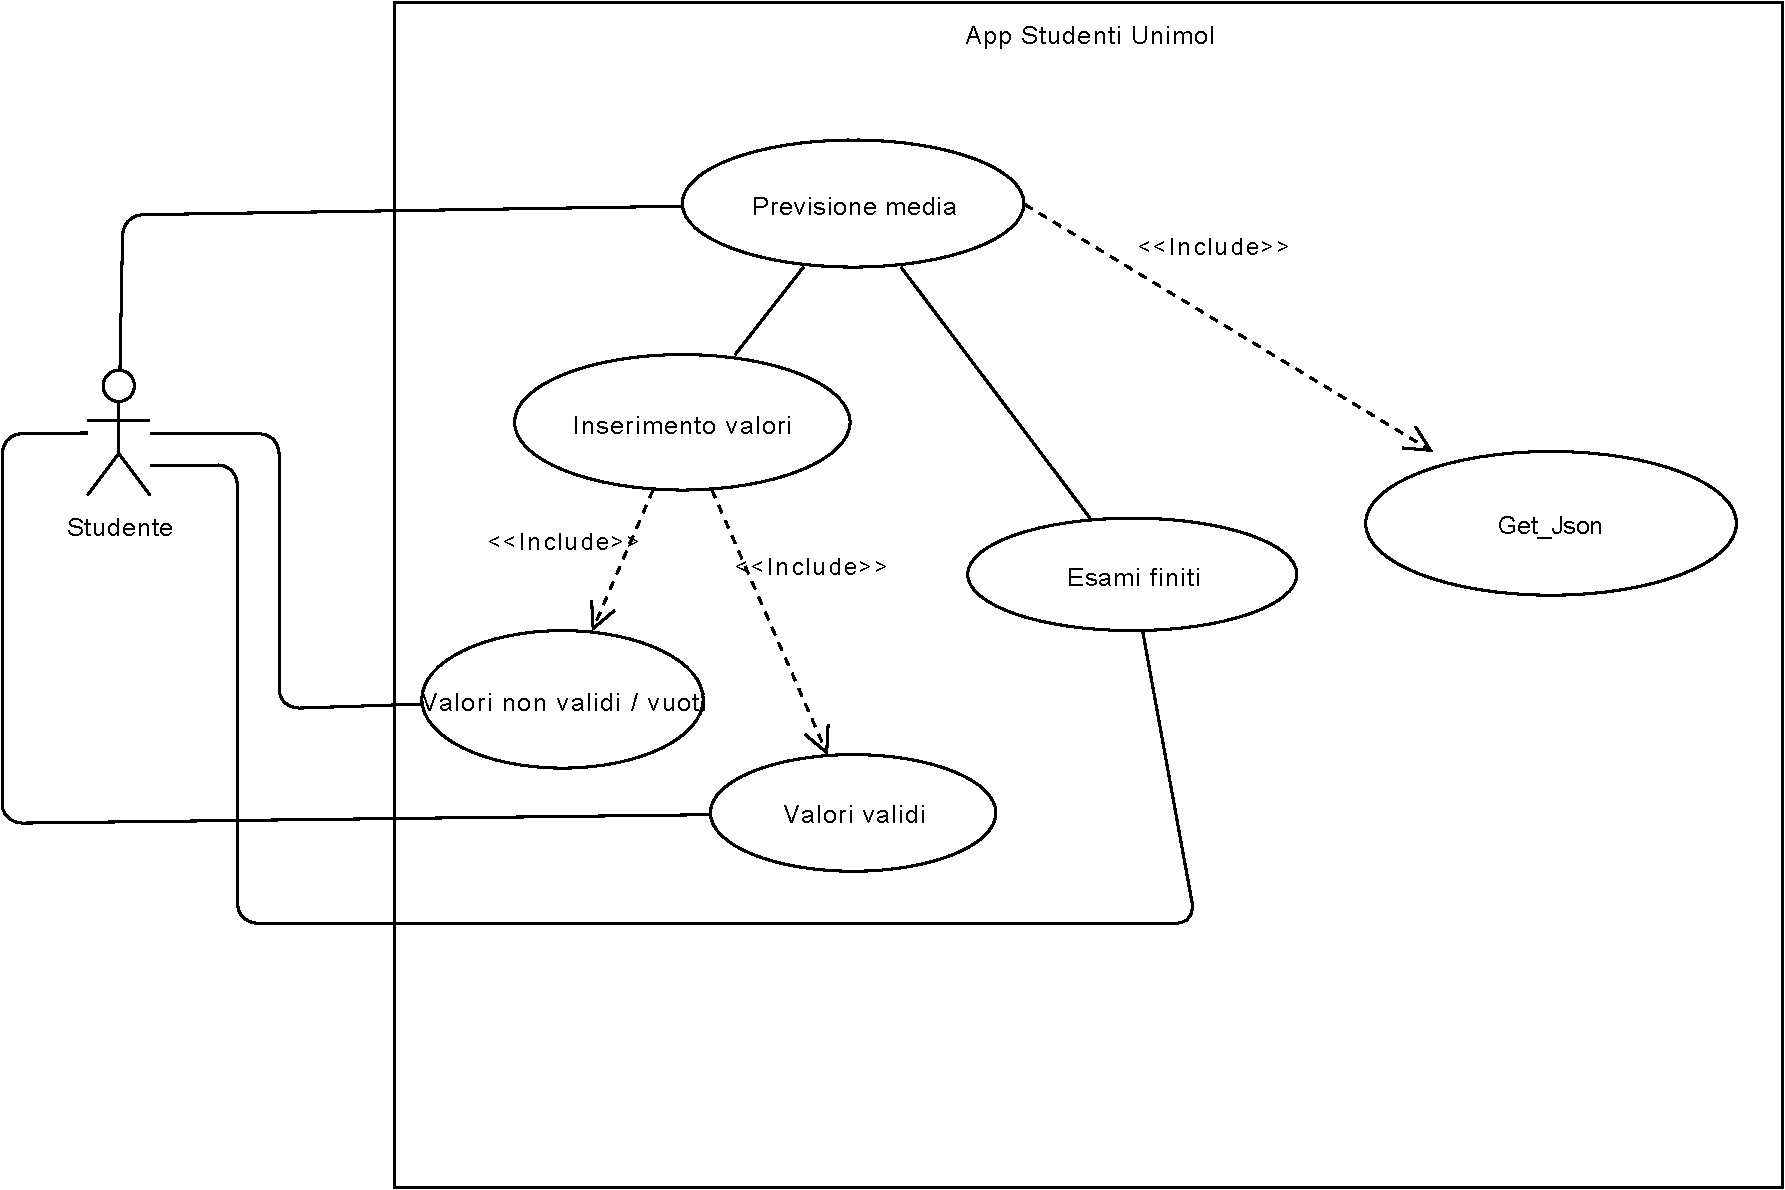
\includegraphics[height=4in]{imgs/gruppo3/caso-duso-media.pdf}
	\caption{caso d'uso media}
	\label{fig:prova}
\end{figure}

\section{Diagrammi di sequenza}
\begin{comment}
Inserire immagine del diagramma. Le immagini vanno caricate nella cartella imgs, va inserito il path corrispondente (nomefile.estensione) dopo il tag includegraphics e va cambiata la descrizione dell'immagine (caption) con un'etichetta opportuna. Sostituire l'immagine file-comuni-ai-gruppi/useCaseEsempio.png con quella desiderata.
\end{comment}
\begin{figure}[H]
	\centering
	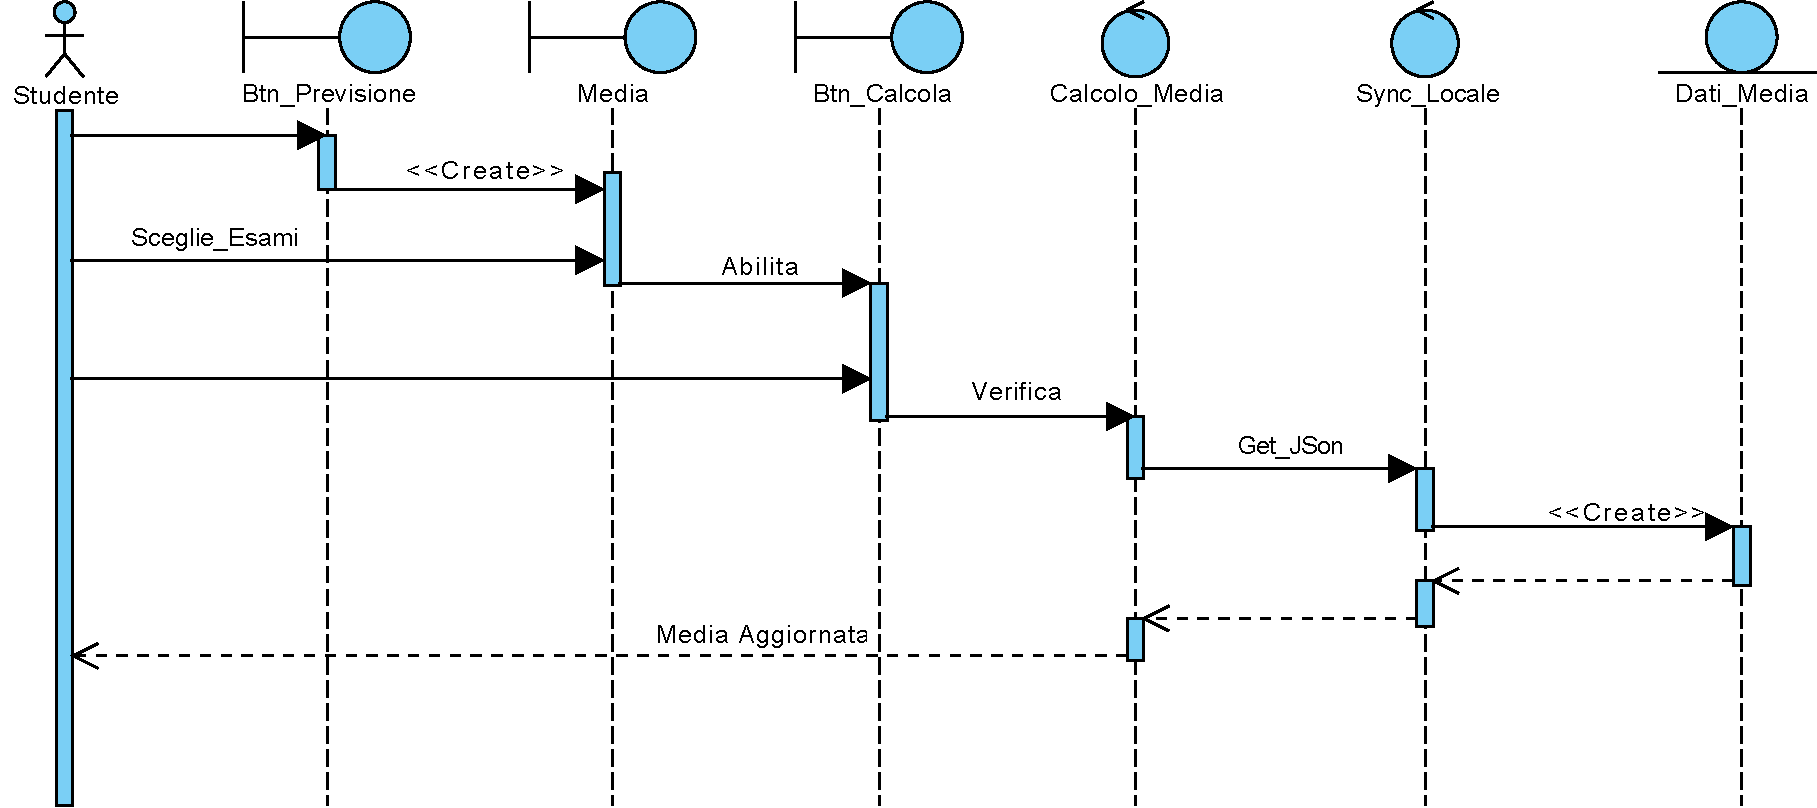
\includegraphics[height=3in]{imgs/gruppo3/sequence-media-valori-validi.pdf}
	\caption{sequence simulazione media}
	\label{fig:prova}
\end{figure}
\begin{figure}[H]
	\centering
	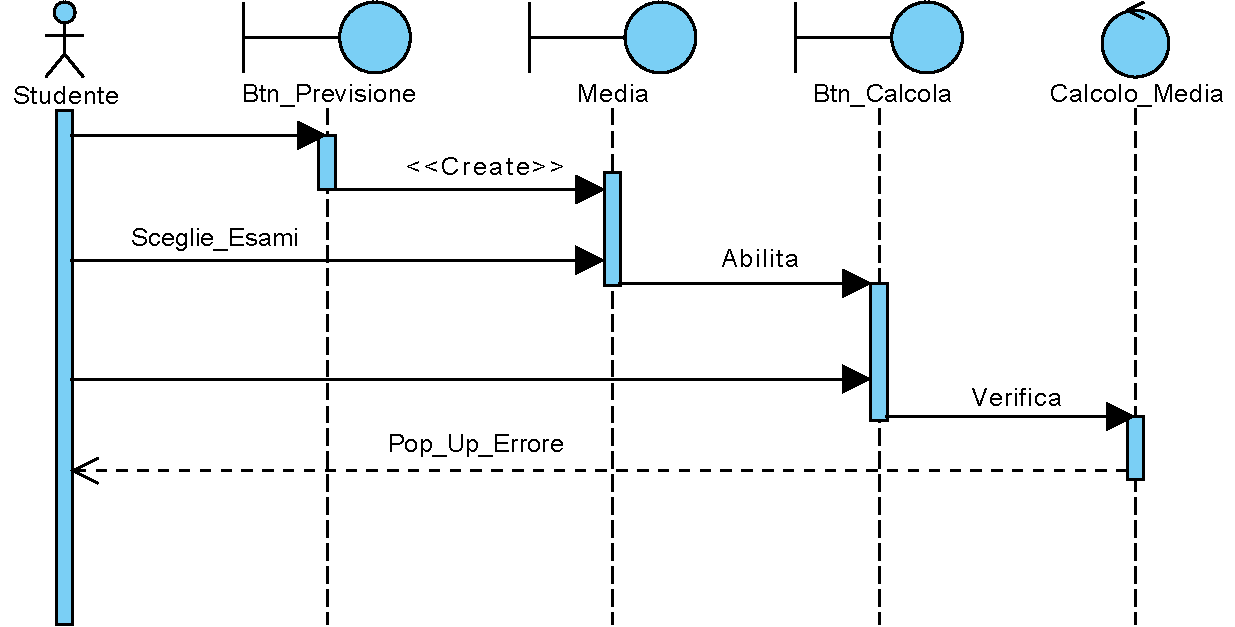
\includegraphics[height=3in]{imgs/gruppo3/sequence-media-valori-non-validi.pdf}
	\caption{Sequence simulazione media con valori non validi o vuoti}
	\label{fig:prova}
\end{figure}
\begin{figure}[H]
	\centering
	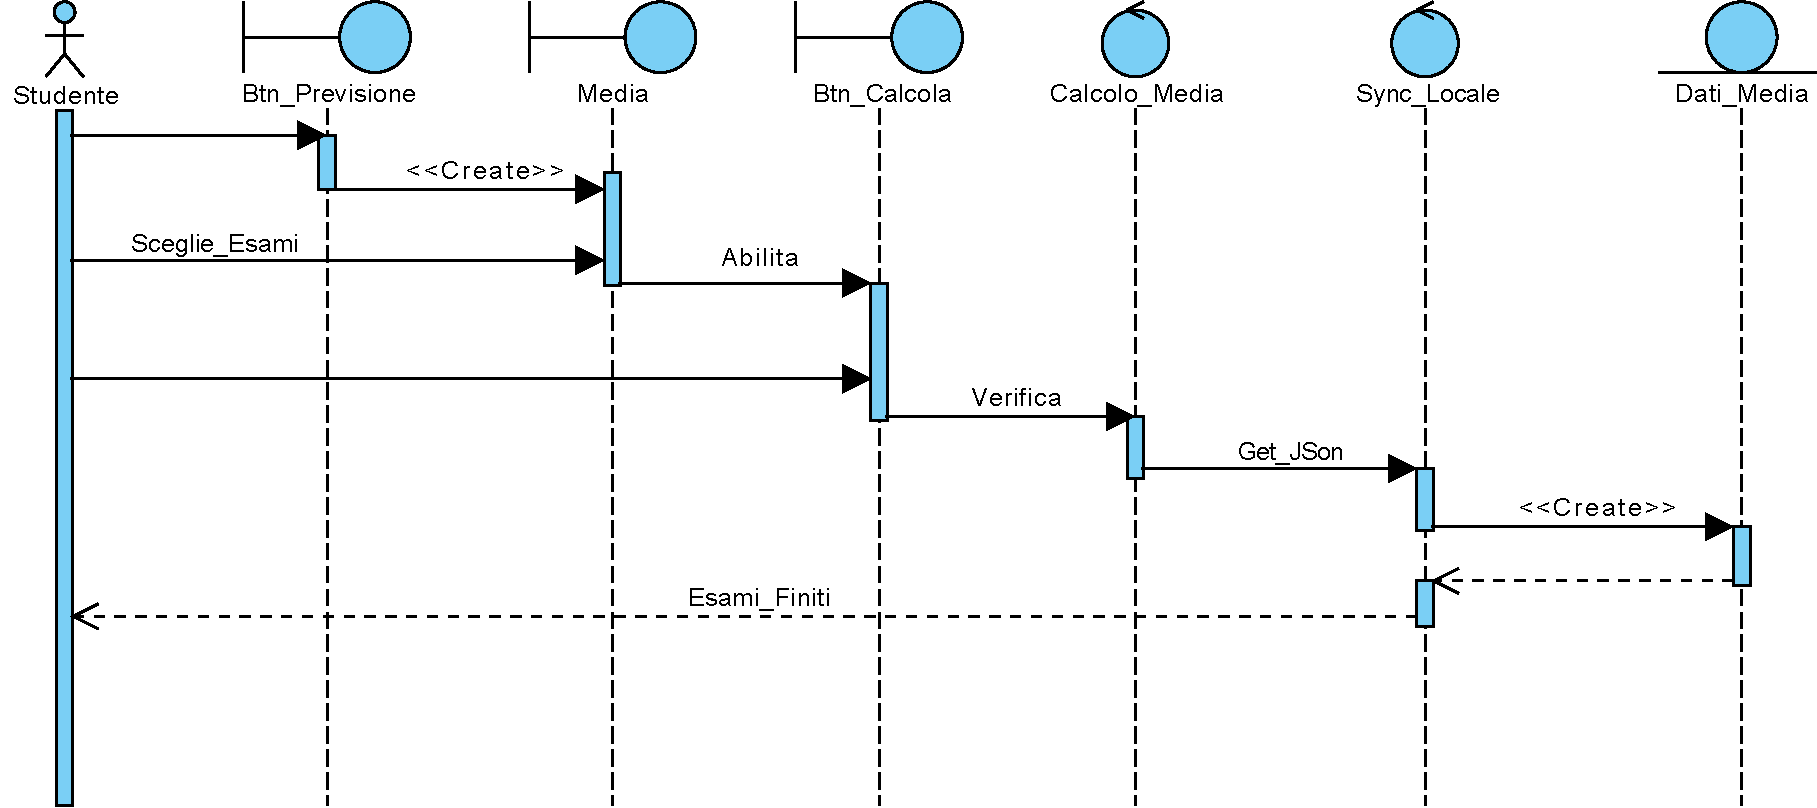
\includegraphics[height=3in]{imgs/gruppo3/sequence-media-esami-finiti.pdf}
	\caption{Sequence simulazione media con esami finiti}
	\label{fig:prova}
\end{figure}

\section{Diagrammi delle attività}
\begin{comment}
Inserire immagine del diagramma. Le immagini vanno caricate nella cartella imgs, va inserito il path corrispondente (nomefile.estensione) dopo il tag includegraphics e va cambiata la descrizione dell'immagine (caption) con un'etichetta opportuna. Sostituire l'immagine file-comuni-ai-gruppi/useCaseEsempio.png con quella desiderata.
\end{comment}
\begin{figure}[H]
	\centering
	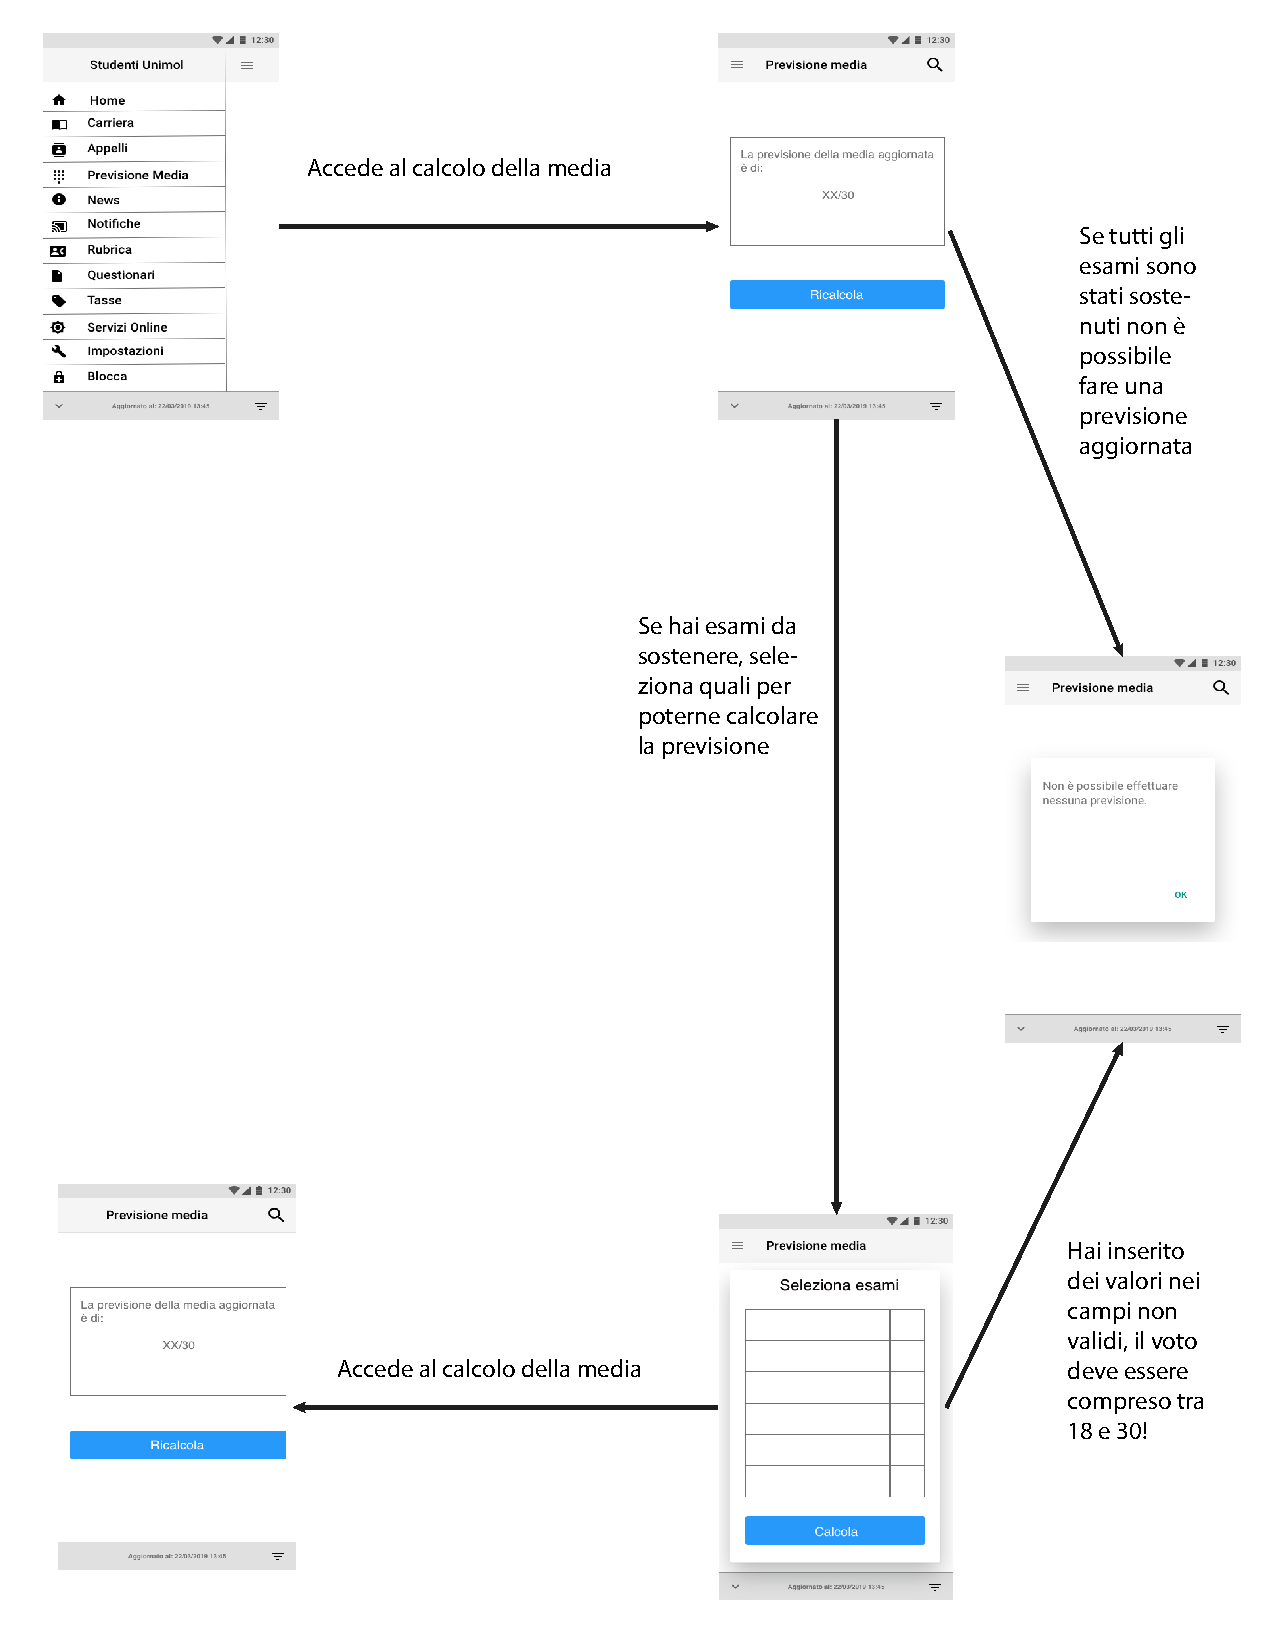
\includegraphics[height=7in]{imgs/gruppo3/media-activity-diagram.pdf}
	\caption{Diagramma di attività}
	\label{fig:prova}
\end{figure}
